\documentclass[a4paper,12pt]{article}
\usepackage{amsmath}
\usepackage{amssymb}
\usepackage[polish]{babel}
\usepackage{polski}
\usepackage[utf8]{inputenc}
\usepackage{indentfirst}
\usepackage{geometry}
\usepackage{array}
\usepackage[pdftex]{color,graphicx}
\usepackage{subfigure}
\usepackage{afterpage}
\usepackage{setspace}
\usepackage{color}
\usepackage{wrapfig}
\usepackage{listings}
\usepackage{datetime}

\renewcommand{\onehalfspacing}{\setstretch{1.6}}

\geometry{tmargin=2.5cm,bmargin=2.5cm,lmargin=2.5cm,rmargin=2.5cm}
\setlength{\parindent}{1cm}
\setlength{\parskip}{0mm}

\newenvironment{lista}{
\begin{itemize}
  \setlength{\itemsep}{1pt}
  \setlength{\parskip}{0pt}
  \setlength{\parsep}{0pt}
}{\end{itemize}}

\newcommand{\linia}{\rule{\linewidth}{0.4mm}}

\definecolor{lbcolor}{rgb}{0.95,0.95,0.95}
\lstset{
    backgroundcolor=\color{lbcolor},
    tabsize=4,
  language=C++,
  captionpos=b,
  tabsize=3,
  frame=lines,
  numbers=left,
  numberstyle=\tiny,
  numbersep=5pt,
  breaklines=true,
  showstringspaces=false,
  basicstyle=\footnotesize,
  identifierstyle=\color{magenta},
  keywordstyle=\color[rgb]{0,0,1},
  commentstyle=\color{Darkgreen},
  stringstyle=\color{red}
  }

\begin{document}

\noindent
\begin{tabular}{|c|p{11cm}|c|} \hline 
Katarzyna Kosiak i Michał Folwarski & \ddmmyyyydate\today \tabularnewline
\hline 
\end{tabular}


\section*{Zadanie 1 - Filtr Gaussa i OpenMP}

Program rozmywa zadane zdjęcie za pomocą algorytmu Gaussa z maską o wymiarach 5x5 korzystając z zadanej liczby wątków.
Zrównoleglono rozmywanie rzędów pikseli zadanego zdjęcia: 
\begin{lstlisting}
#pragma omp parallel num_threads(numberOfThreads)
    {
    	for (int i = offset; i <= rows - offset -1; i++) {
    	        for (int j = offset; j <= cols - offset -1; j++) {
    	        	 /obliczanie nowych wartosci RGB dla piksela
    	        }
    	    }
    }
\end{lstlisting}
W powyższym fragmencie użyto zmiennej offset, która wynosi 3 (dla maski o rozmiarze 5x5) i powoduje ominięcie brzegowych pikseli obrazu.

Poniższy wykres pokazuje zależność czasu działania programu od liczby wątków dla przykładowego obrazu: \\
\begin{figure}[h]
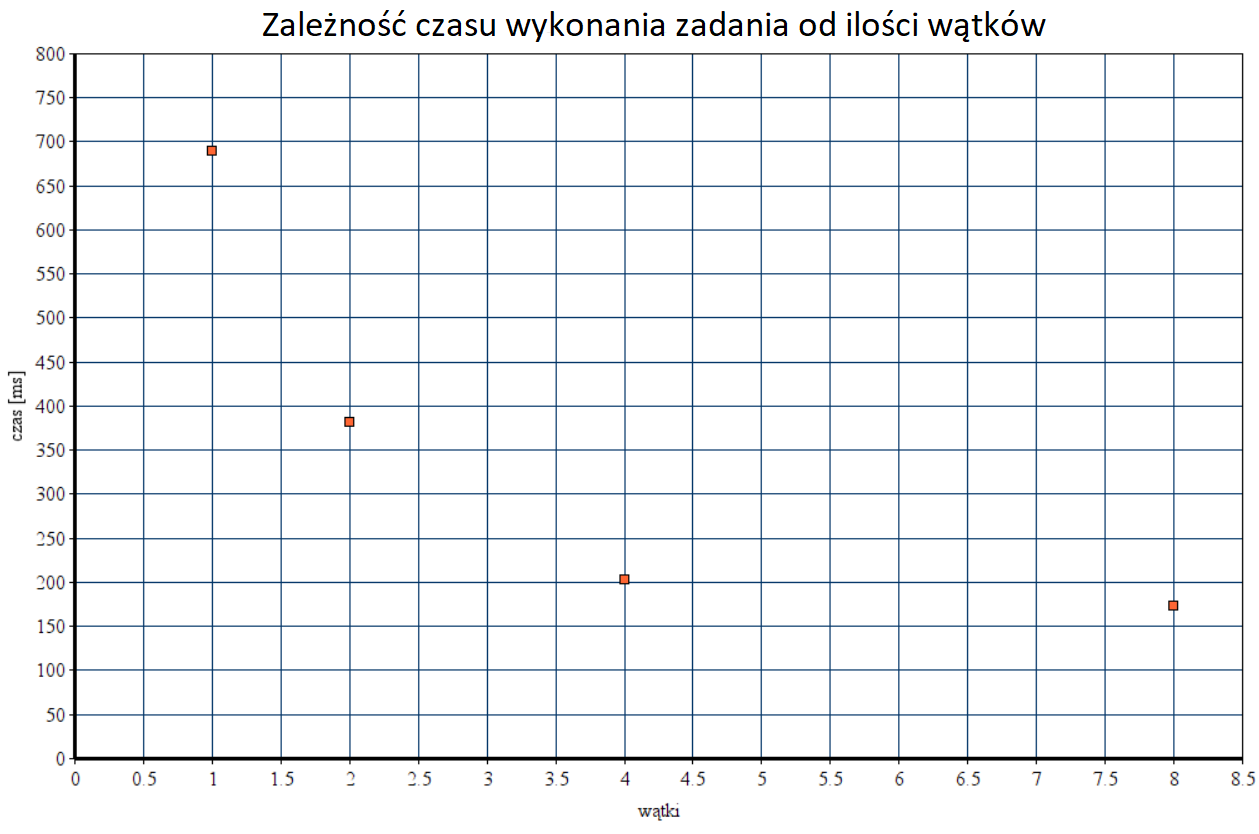
\includegraphics[width=15cm]{wykres_zad1}
\end{figure}


W celu ułatwienia pracy Prowadzącemu warto wykresy podpisać, aby Prowadzący omyłkowo nie przyjął, że dany wykres przedstawia średnią miesięczną temperaturę w Bangladeszu na przełomie lat 1975-1982, ponieważ taki wykres byłby nieodpowiedni, przez co sprawozdanie byłoby niezaliczone. Łatwo zauważyć, że każdy wykres w przestrzeni 2D posiada dwie osie i z grzeczności należy je opisać. Osie posiadają jednostki, które też warto przytoczyć.

Zalety tego rozwiązania to: TODO
\begin{lista}
 \item Pierwszą zaletą jest to, że jest.
 \item Druga zaleta jest również obecna.
\end{lista}

Wnioski
TODO

W sprawozdaniu muszą znaleźć się wnioski. Wnioski stanowią przesłankę, o tym iż osoba je pisząca, która ubiega się o tytuł magistra inżyniera, wie co robi. Osoba taka często jest w stanie określić czemu miało służyć dane ćwiczenie, a także ocenić w jakim stopniu udało się rozwiązać dane zagadnienie i gdzie napotkano problemy.

\end{document}
